\section{Analysis}
\label{sec:Analysis}
At first, the invariant mass distributions of the reconstructed \printBdstoPsiKs are inspected for the simulation and real data.
In \autoref{fig:mass_signal}, the invariant mass distribution of the reconstructed $B^0_s$ events in the signal simulation is shown.
As expected, a clear peak at the $B^0_s$ mass can be seen.
\begin{figure}
  \centering
  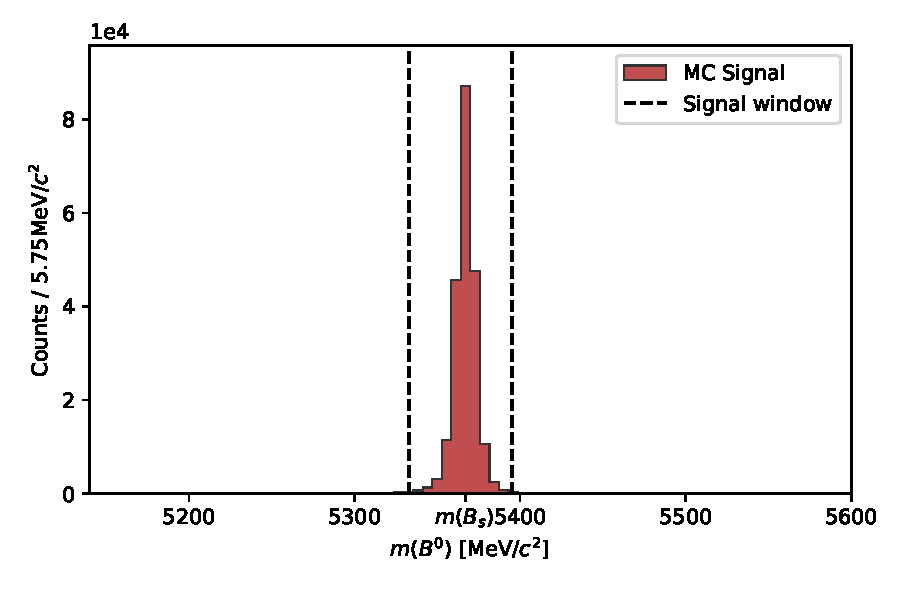
\includegraphics[width = .8\textwidth]{"content/plots/mass_signal.pdf"}
  \caption{Invariant mass distribution of the $B^0_s$ candidates for the signal channel simulation data.}
  \label{fig:mass_signal}
\end{figure}
The mass distribution of the reconstructed $B^0$ candidates in real data can be seen in \autoref{fig:mass_data}. Here, a peak at the nominal $B^0$ mass can be seen. However,
due to dominating combinatorial background, no peak at the $B^0_s$ mass is visible.
\begin{figure}
  \centering
  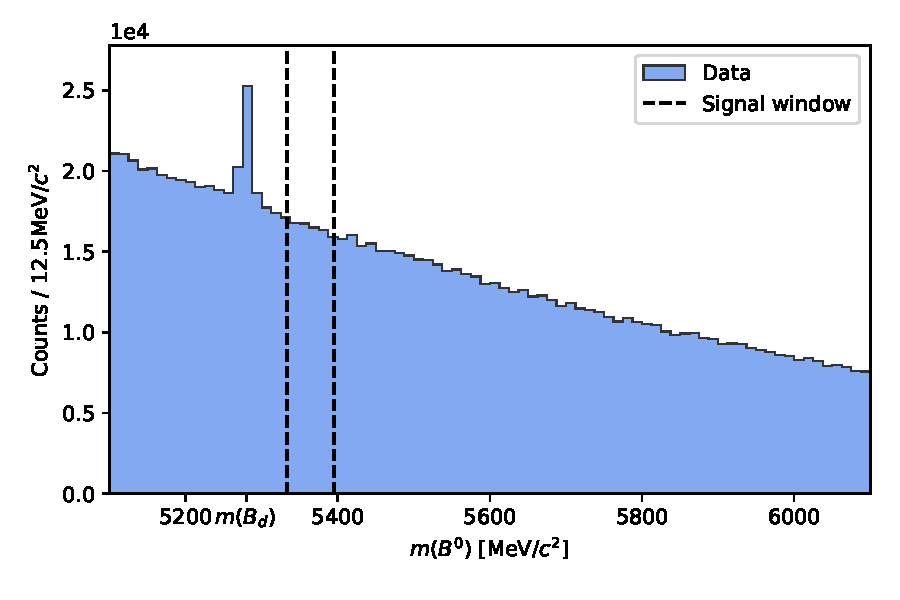
\includegraphics[width = .8\textwidth]{"content/plots/mass_data.pdf"}
  \caption{Invariant mass distribution of the $B^0$ candidates for the recorded LHCb data.}
  \label{fig:mass_data}
\end{figure}
The dataset also contains \textit{sWeights} which can be used to extract the contribution of the control channel in the dataset.
By weighting the mass histogram with the sWeights, only the control channel contribution remains in the plot, as can be seen in \autoref{fig:mass_reweighted}.
\begin{figure}
  \centering
  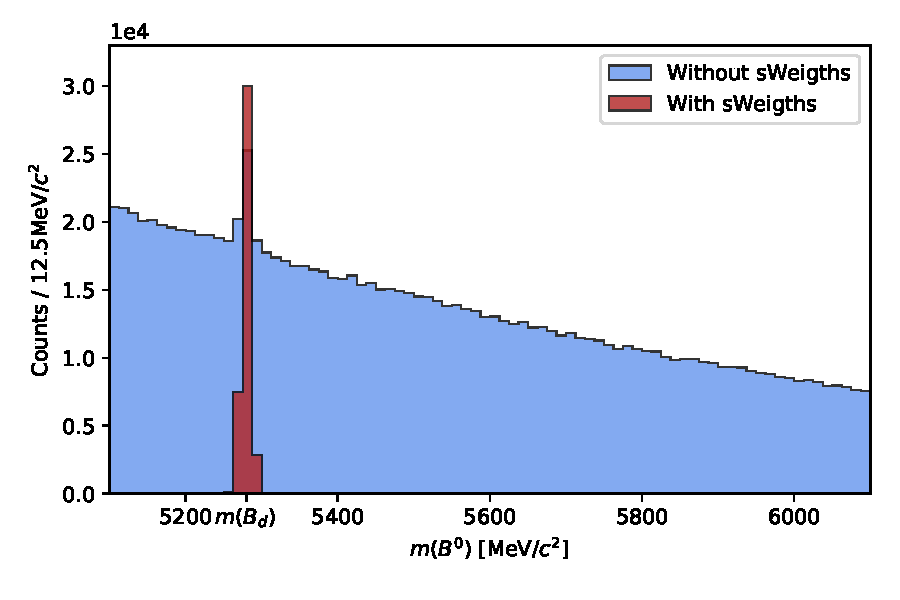
\includegraphics[width = .8\textwidth]{"content/plots/mass_reweighted.pdf"}
  \caption{Invariant mass distribution of the $B^0$ candidates for the recorded LHCb data with and without the sWeights.}
  \label{fig:mass_reweighted}
\end{figure}

\subsection{Definition of a signal window}
The mass distribution of the signal decay peaks only in a short window of the whole mass range given in the dataset. In order to know, where signal is expected, a signal window 
has to be defined. This is done by calculating every interval containing $\qty{99}{\percent}$ of data in the signal simulation and choosing the shortest interval. 
Here, this interval follows as $\qtyrange[range-units = single]{5333.4}{5394.6}{\mega\eVperc}$, defining the signal window of 
$\qtyrange[range-units = single]{5333}{5395}{\mega\eVperc}$ which can also be seen in the aforementioned plots (\ref{fig:mass_signal}, \ref{fig:mass_data}).
Subsequently, the upper sideband (\enquote{\textit{USB}}), containing mostly combinatorial background, is defined as the area with reconstructed mass $> \qty{5400}{\mega\eVperc}$.

\subsection{Feature selection}
In order to train a multivariate classifier capable of separating signal from background, meaningful features from all available variables in the dataset 
have to be selected. In total, $\num{863}$ variables are listed in the dataset. After removing event, utility, trigger and spatial coordinate variables, $\num{398}$ variables remain.
For these variables, the correlation to the invariant mass is calculated and variables having a correlation coefficient of $\num{0.3}$ or higher are excluded.
Variables with too high correlation to the invariant mass would introduce a bias in training the classifier and could not be used in similarity checks between simulation and data,
because the sWeights are based on the $B^0$ candidate mass. The remaining $\num{390}$ variables are checked to be correctly modelled by simulation and have significantly different 
distributions for signal and background. This is done using the Kolmogorov Smirnov test statistic defined in \autoref{eq:Kolmogorov} for weighted distributions as a measure of similarity. 
To check agreement between simulation and data, the distributions of sWeighted data are compared to the control channel distributions and 
only variables with a test statistic of $d < \num{0.05}$ are kept. $\num{190}$ variables with a higher test statistic are removed. 
The variables are also required to have a test statistic of $d > \num{0.2}$ when comparing signal (simulation) and background (USB), leaving 
$\num{94}$ variables. After further removing variables that are highly correlated (correlation $> 0.9$) to others or dublicates of another variable, $\num{18}$ variables are 
left that are used for the training of the multivariate classifier.
\begin{figure}
  \centering
  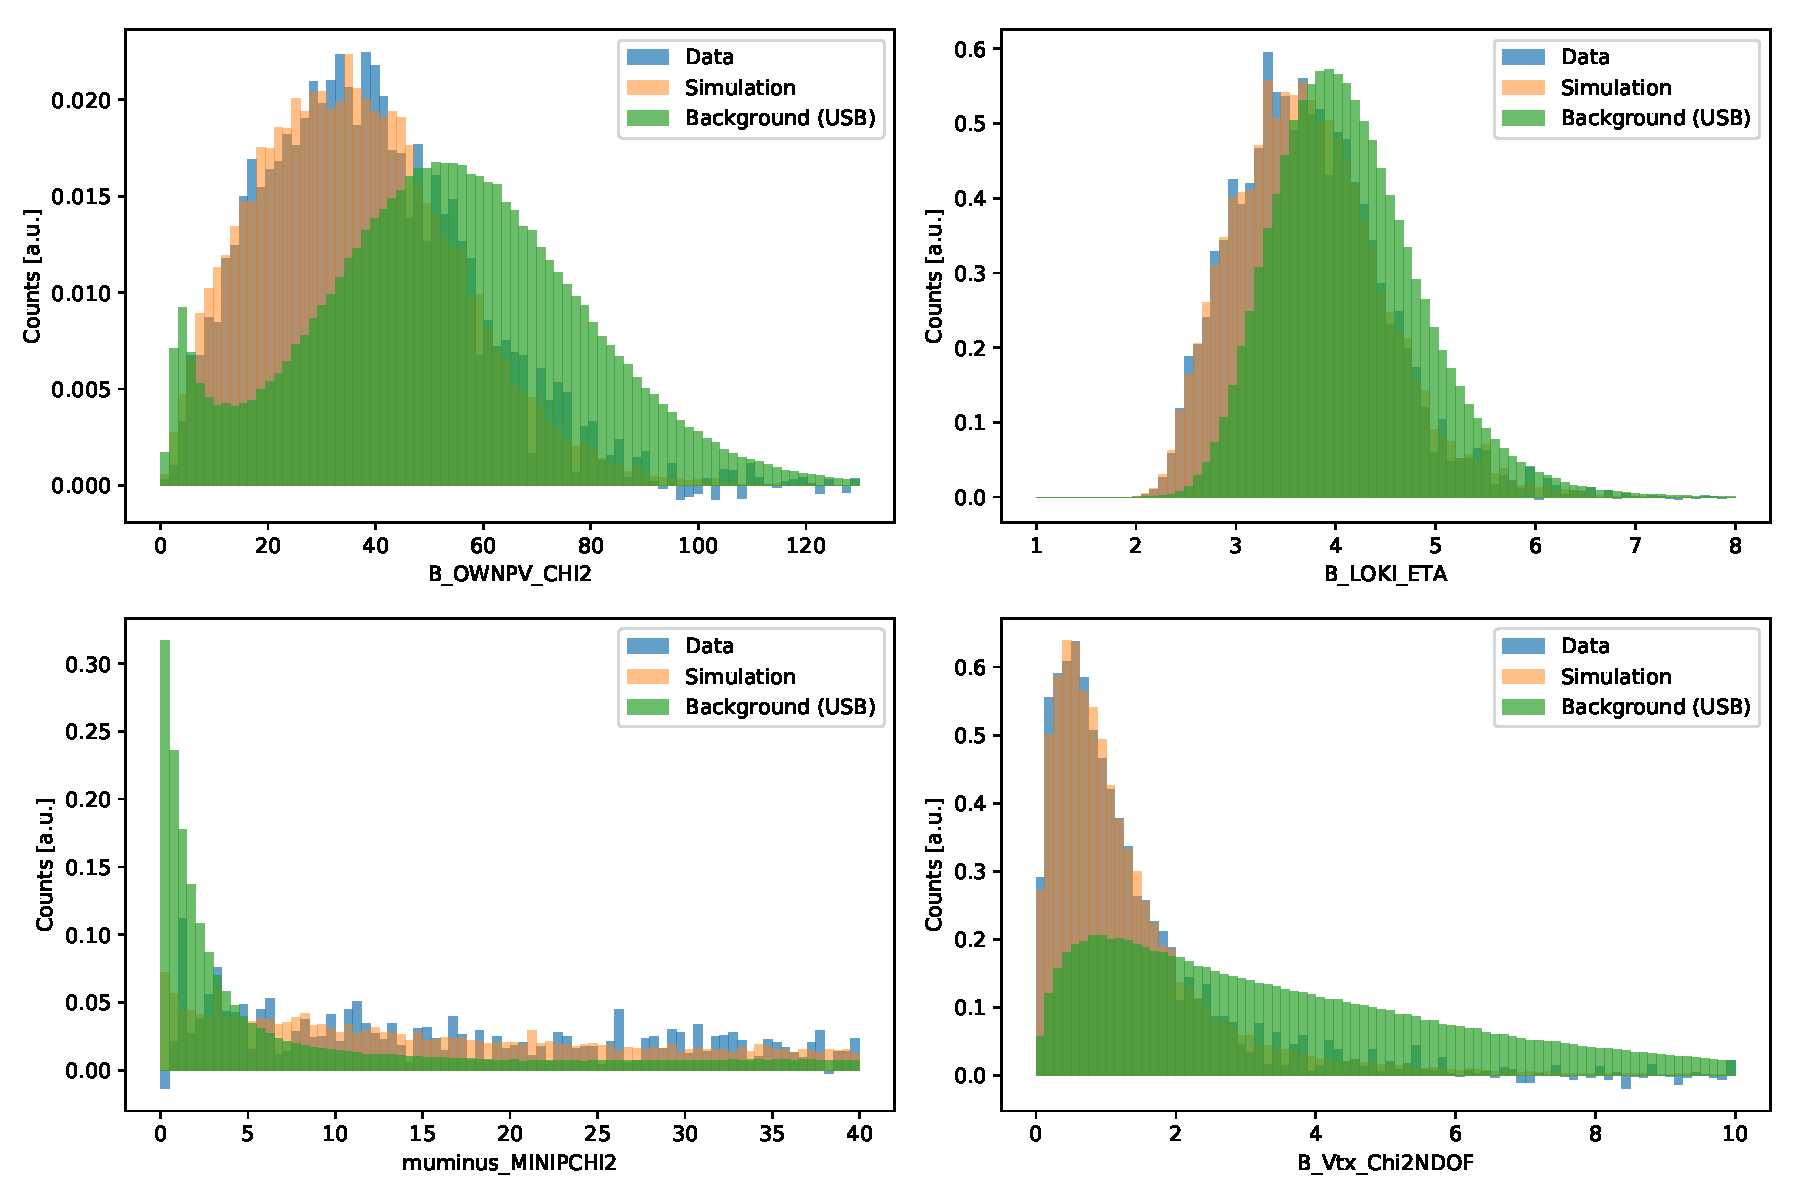
\includegraphics[width = .9\textwidth]{"content/plots/4variables.pdf"}
  \caption{Distributions of four selected variables used in the MVA for simulation, reweighted data and background.}
  \label{fig:4variables}
\end{figure}
The distributions of four of these variables for signal and background, as well as control channel data and simulation are shown in \autoref{fig:4variables}. Distributions for all
variables and the correlation matrix can be found in the appendix \ref{sec:Appendix1}.

\subsection{Training of a multivariate classifier}
With the now selected variables, a multivariate classifier can be trained. For this purpose, a boosted decision tree as implemented in the package \texttt{XGBoost} \cite{XGBoost}
is used. The training data consists of $\num{637410}$ background events and kinematically reweighted signal simulation, corresponding to $\num{155805}$ events. Because of this 
inbalance, each background event is weighted with a factor of $155805/637410$.
The hyperparameters of the classifier are optimized via a random search followed by a grid search using cross validation and a subset of $\num{40000}$ training samples. 
The resulting parameter values can be read from \autoref{tab:hyperparameter}.
\begin{table}[h!]
  \centering
  \caption{Hyperparameter values of the trained classifiers determined by grid search.}
  \label{tab:hyperparameter}
  \begin{tabular}{c | c}
    \hline
    {Parameter} & {Value} \\
    \hline
    \texttt{n\_estimators} & {$\num{1000}$} \\
    \texttt{learning\_rate} & {$\num{0.1}$} \\
    \texttt{max\_depth} & {$\num{4}$} \\
    \texttt{reg\_lambda} & {$\num{1}$} \\
    \texttt{n\_iter\_no\_change} & {$\num{5}$} \\
    \hline   
  \end{tabular}
\end{table}
For the classification, five individual BDT's are trained using 5-fold cross validation and the hyperparameters from \autoref{tab:hyperparameter}.
To evaluate the classifiers performance, the ROC curve is viewed and the area under the curve, as well as the accuracy are calculated. 
To check for overtraining, the response of the classifier is compared for training and simulation data in a logarithmic plot.
The ROC curve and the train-test comparison of the fifth trained classifier can be seen in \autoref{fig:BDT}.
\begin{figure}
  \centering
  \begin{subfigure}[b]{0.45\textwidth}
    \centering
    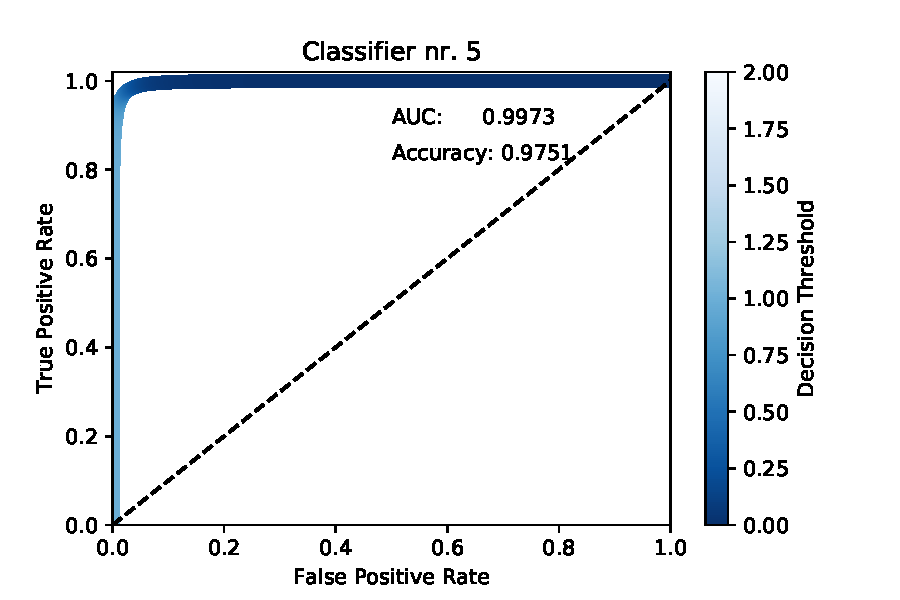
\includegraphics[width=\textwidth]{"content/plots/BDT/BDT_roc_auc4.pdf"}
    \caption{ROC curve.}
    \label{fig:roc_curve}
  \end{subfigure}
  \hfill
  \begin{subfigure}[b]{0.45\textwidth}
    \centering
    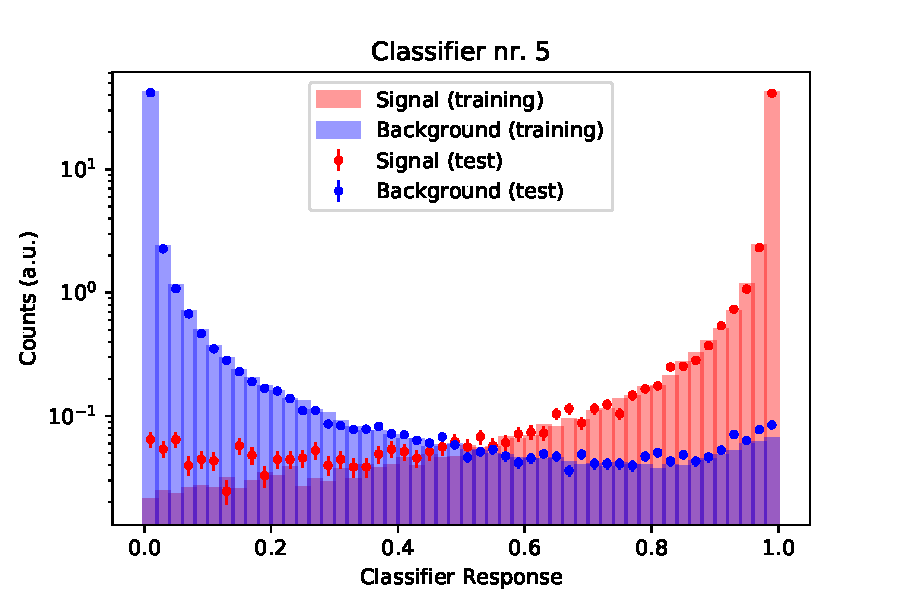
\includegraphics[width=\textwidth]{"content/plots/BDT/BDT_train_test4.pdf"}
    \caption{Performance on test vs. training dataset.}
    \label{fig:train_test}
  \end{subfigure}
  \caption{ROC curve (left) and response on training and test dataset (right) for one of the trained classifiers.}
  \label{fig:BDT}
\end{figure}
Additionally, the feature importance of the BDT variables is checked for imbalances. As can be seen in \autoref{fig:feature_importance}, all variables are of similar importance.
\begin{figure}
  \centering
  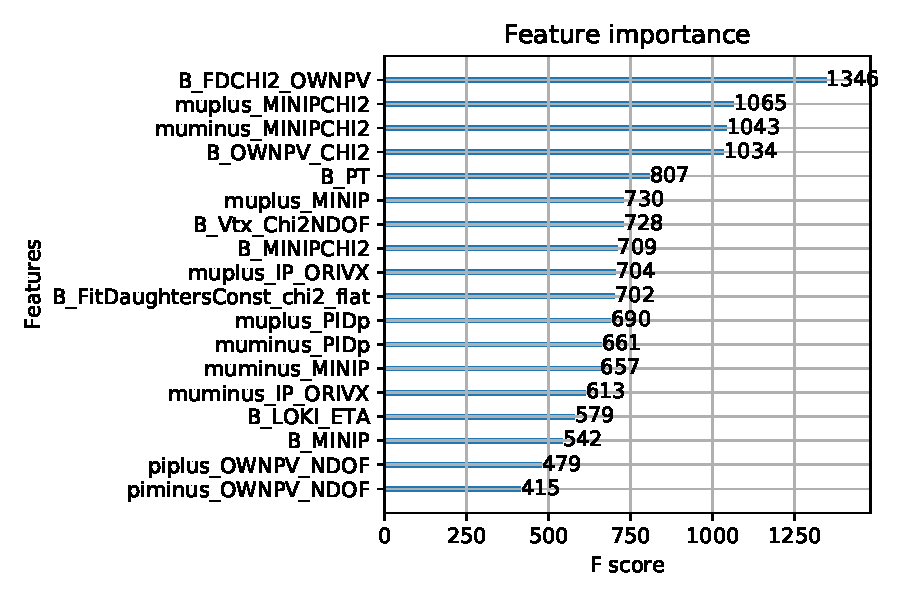
\includegraphics[width = .7\textwidth]{"content/plots/BDT/feature_importance.pdf"}
  \caption{Feature importance of the BDT training variables.}
  \label{fig:feature_importance}
\end{figure}


\subsection{Optimization of the classification threshold}
After applying all BDT's to the data, a cut on the classifiers response has to be made. Therefore the mean classifier response between all 5 BDT's is calculated.
The classification threshold separating signal and background is optimized using the Punzi figure of merit \autoref{eq:FOM}.
The signal efficiency $\varepsilon$ is therefore calculated for each threshold as the selection efficiency on the signal simulation. The background yield in the signal region $B$
is estimated via a fit of an exponential function to the upper sideband of the data after applying the selection threshold, and extrapolated to the signal window.
For the fitting, the python library \texttt{iminuit} \cite{iminuit} is used.
The resulting values of the figure of merit are plotted against different thresholds in \autoref{fig:pFOM}.
\begin{figure}
  \centering
  \begin{subfigure}[b]{0.45\textwidth}
    \centering
    \includegraphics[width=\textwidth]{"content/plots/pfom_full.pdf"}
    %\caption{ROC curve.}
  \end{subfigure}
  \hfill
  \begin{subfigure}[b]{0.45\textwidth}
    \centering
    \includegraphics[width=\textwidth]{"content/plots/pfom_zoom.pdf"}
  \end{subfigure}
  \caption{The Punzi figure of merit for the mean classifier response in different intervals of the threshold.}
  \label{fig:pFOM}
\end{figure}
The optimal classification threshold is the maximum value of the Punzi figure of merit and reads as $t = 0.998$.

\subsection{Evaluation of the signal yield}
The invariant $B^0$ mass distribution of the data after applying the cut on the mean BDT response can be seen in a semi-logarithmic plot in \autoref{fig:mass_after_BDT}.
\begin{figure}
  \centering
  \includegraphics[width = .8\textwidth]{"content/plots/mass_after_BDT.pdf"}
  \caption{Semi logarithmic invariant mass distribution of the $B^0$ candidates in data, after the cut on the classifier response is applied.}
  \label{fig:mass_after_BDT}
\end{figure}
%A peak of the signal decay \pritBstoPsiKs \: can be seen.
In the mass region below $\qty{5150}{\mega\eV}$, a prominent background band of partially reconstructed decays can be seen.

In order to determine the signal yield, a fit to the mass spectrum of the $B^0$ candidates is applied.
The fit range is defined as $\qty{5200}{\mega\eV} < m(B^0) < \qty{6100}{\mega\eV}$ to not include the partially reconstructed background.
The signal peaks are modeled with two gaussian distributions with a fixed width ratio $\alpha$ which is determined from simulation.
Using this definition, the width of the $B^0$ peak is given by $\sigma_0$ and the width of the $B^0_s$ peak by $\sigma_0 \cdot \alpha$.
The values of the width $\sigma_0$ and the mean values $\mu_{B_d}, \mu_{B_s}$ of the gaussian distributions are allowed to vary freely to account 
for mass resolution differences in data and simulation. 
The background is again modeled by an exponential function with decay constant $\tau$.
An extended, unbinned negative Log-Likelihood fit is performed, including the fractions $s_{B_d}, s_{B_s}$ and $b$ of signal, control channel and background components.
The resulting graph is shown in \autoref{fig:fit}.
\begin{figure}
  \centering
  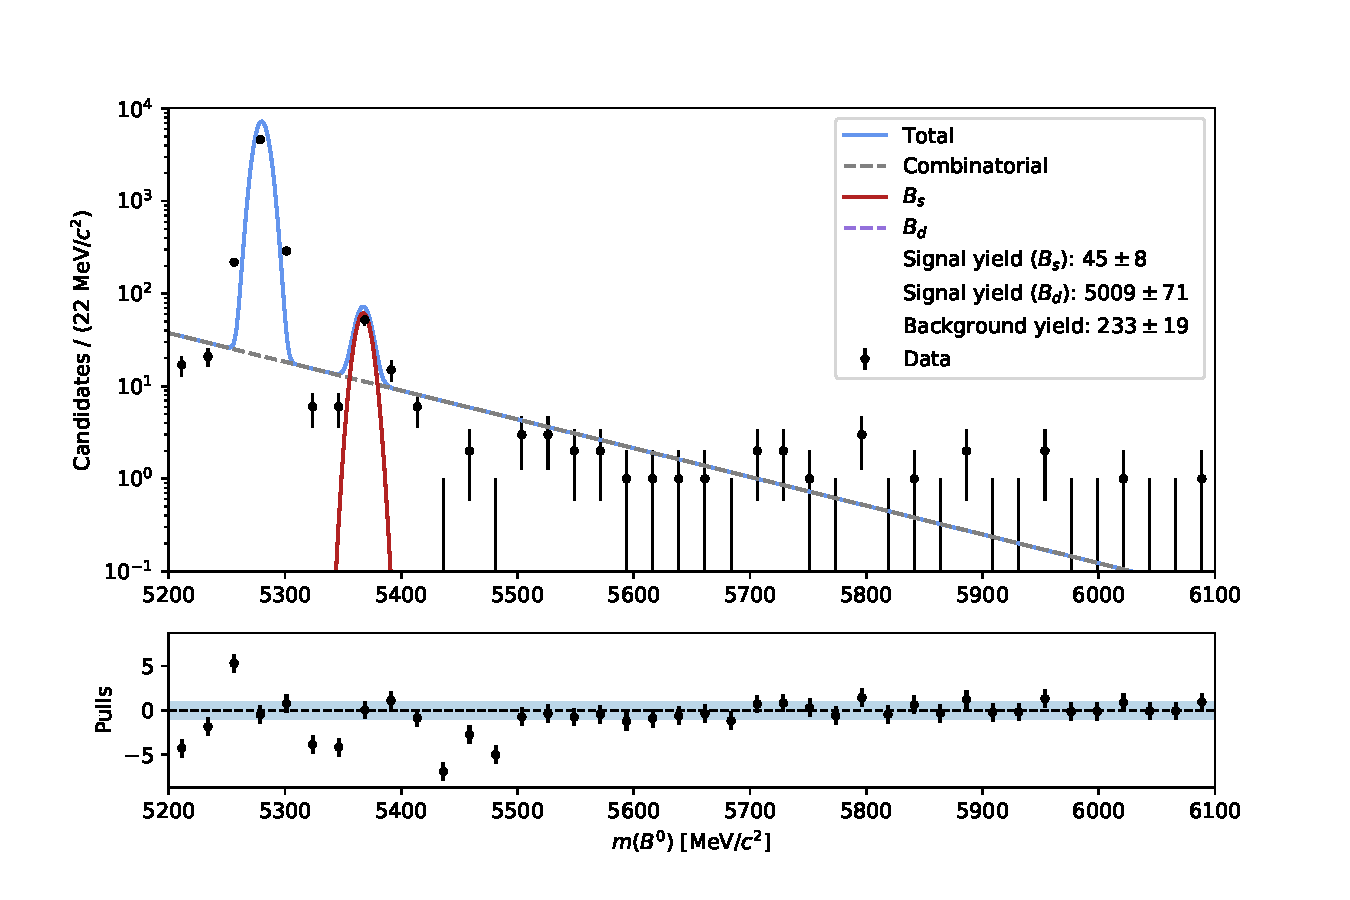
\includegraphics[width = .9\textwidth]{"content/plots/final_fit.pdf"}
  \caption{Fit to the invariant mass spectrum of the data in semi logarithmic depiction.}
  \label{fig:fit}
\end{figure}
The fit parameters follow as 
\begin{align*}
  s_{B_s} &= \num{45 +- 8} & s_{B_d} &= \num{5010 +- 70} \\
  \mu_{B_s} &= \qty{5367.3 +- 1.2}{\mega\eVperc} & \mu_{B_d} &= \qty{5279.9 +- 0.9}{\mega\eVperc} \\
  \sigma_{0} &=  \qty{6.21 +- 0.08}{\mega\eVperc} & \alpha &=  \num{1.056 +- 0.011} \\
  b &= \num{233 +- 19}  & \tau &= \num{140 +- 10}.
\end{align*}
From these, the significance as defined in \autoref{eq:sign} of the observation of the signal can be calculated.
Therefore, the signal and background events in the signal window are interpolated from the fit results as $n_\text{sig} = \num{45}$ and $n_\text{bkg} = \num{32}$.
The significance proxy then reads $m = \num{5.1}$.
